% =============================================================================
%  Section: Unfolding
%  H1 Charged-Hadron SIDIS High-Q^2 Analysis Note
% =============================================================================
\section{Unfolding}
\label{sec:unfolding}

The binning of the analysis in $Q2,x,z,$ and $\pTh$ was selected to have an acceptable purity and acceptance in almost all bins. The purity is defined as $N_{\mathrm{stay}}/N_{\mathrm{rec}}$, where $N_{\mathrm{rec}}$ includes the fake column. The acceptance is defined as $N_{\mathrm{rec}}/N_{\mathrm{gen}}$.

The response basis for these metrics is RAPGAP31 with the current release
selection: the detector-interaction-corrected response together with the
reconstruction-only $\alpha<0.2$ scattered-electron cone
veto after the electron and V0 truth vetoes and before the $z$ guard.  The
generator side is unchanged; cone-rejected matched legs flow to the miss row.
The current-hemisphere requirements are $xF_{\mathrm{SIDIS\_es}}<0$ at
reconstruction level and $xFGen<0$ at generator level; generator-level $x_F$
is recomputed with the $q$-nominal construction. The IBU prior is the
response's own generator-level truth distribution, computed from this
response.

The worst purities are found in the higher $x$ strata at high $\pTh$, where the minimum value is 3.0\%. At high-$x$, the resolution on the virtual photon is generally worse, resulting in large migrations from the much more populated low-$\pTh$ region to the high-$\pTh$ tail. The systematic uncertainties on these bins are very large, and they may be dropped from the final set of published bins. The purities for $h^+$ and $h^-$ are shown in Figs.~\ref{fig:unfolding:alpha0p2-purity} and~\ref{fig:unfolding:alpha0p2-purity-hm}, respectively. The worst acceptances are found in the low-$z$, high $\pTh$ region, where the tracks predominantly fall at $\eta>1.6$ in the lab frame.

The nominal unfolding method is the D'Agostini-style Iterative Bayesian Unfolding (IBU) implemented in RooUnfold, using $k=4$ iterations; bin-by-bin correction is retained as a cross-check. TUnfold is presented as a diagnostic comparison candidate and is not an alternative central result. Both methods carry uncertainties associated with the model-dependence of the migration matrix, limited data and/or MC statistics, and the choice of arbitrary parameters ($\tau$ for TUnfold and $N_{\mathrm{iter.}}$ for IBU). The uncertainties will be described in more detail in Sec.~\ref{sec:systematics}.

For the diagnostic TUnfold comparison, the migration matrix is produced with twice the number of reconstruction-level bins in $\pTh$ to help the unfolding better deal with migrations. To reduce the size of the matrix, $h^+$ and $h^-$ are unfolded separately, only 0.19\% of tracks are reconstructed with the wrong charge, so this is a reasonable approximation\footnote{This should be compared to the 2020 analysis, where each kinematic bin was unfolded separately.}. Charge-confused tracks are treated as misses in one matrix and fakes in the other. $\pTh$ was chosen as the variable to bin more finely since it experiences the largest migration. Unfolding with larger numbers ($>2\times$) of reconstruction-level bins gave similar results at the cost of significantly larger compute time. The value of the regularization strength, $\tau$, in TUnfold was chosen to minimize correlations between bins as well as the model, statistical, and regularization uncertainties. The model uncertainty is defined as the difference between the data unfolded with the Rapgap migration matrix and the data unfolded with the Djangoh migration matrix. One challenge with TUnfold is that in the high-$\pTh$ bins where data statistics are low, some bins occasionally unfold to a negative cross section.

The IBU unfolding does a good job of reproducing the truth of Rapgap when the reconstruction-level Rapgap data is unfolded with the Djangoh migration matrix, and vice versa. IBU also provides stable results for most bins at any value of $N_{\mathrm{iter.}}<10$. IBU and TUnfold generally agree quite well, with the exception of some edge bins where TUnfold produces oscillations.

Figure~\ref{fig:unfolding:alpha0p2-allfake-migration-matrix} shows the diagnostic all-fake response used for the provisional near-electron opening-angle veto study. The positive- and negative-charge response matrices each have shape $(491,246)$: rows 0--489 are physical reconstructed bins and row 490 is the miss row, while columns 0--244 are physical truth bins and column 245 is the fake column. The response is shown without stretching of the fake or miss bins and is column-normalized as $P(\mathrm{reco\ bin}\mid\mathrm{truth\ bin})$ on a logarithmic colour scale. This all-fake response is diagnostic and provisional only; central response and release products were not overwritten.

The IBU cross-generator closure diagnostic is shown in Figs.~\ref{fig:unfolding:ibu-crossclosure-fullrange} and~\ref{fig:unfolding:ibu-crossclosure-zoom}. These plots use the canonical seven-column $\pTh$ layout and include both cross directions, with $\mathrm{DJ}\to\mathrm{RG}=N^{\mathrm{DJ\ reco,\ unfolded\ with\ RG\ response}}/N^{\mathrm{DJ\ truth}}$ and $\mathrm{RG}\to\mathrm{DJ}=N^{\mathrm{RG\ reco,\ unfolded\ with\ DJ\ response}}/N^{\mathrm{RG\ truth}}$. The comparison is a cross-generator closure check only, with no self-closure component; the full-range version displays ratios from 0 to 2 and the zoomed version displays 0.75 to 1.25. These figures are note-ready diagnostics derived from the validated cross-closure input table.

\begin{figure}[t]
  \centering
  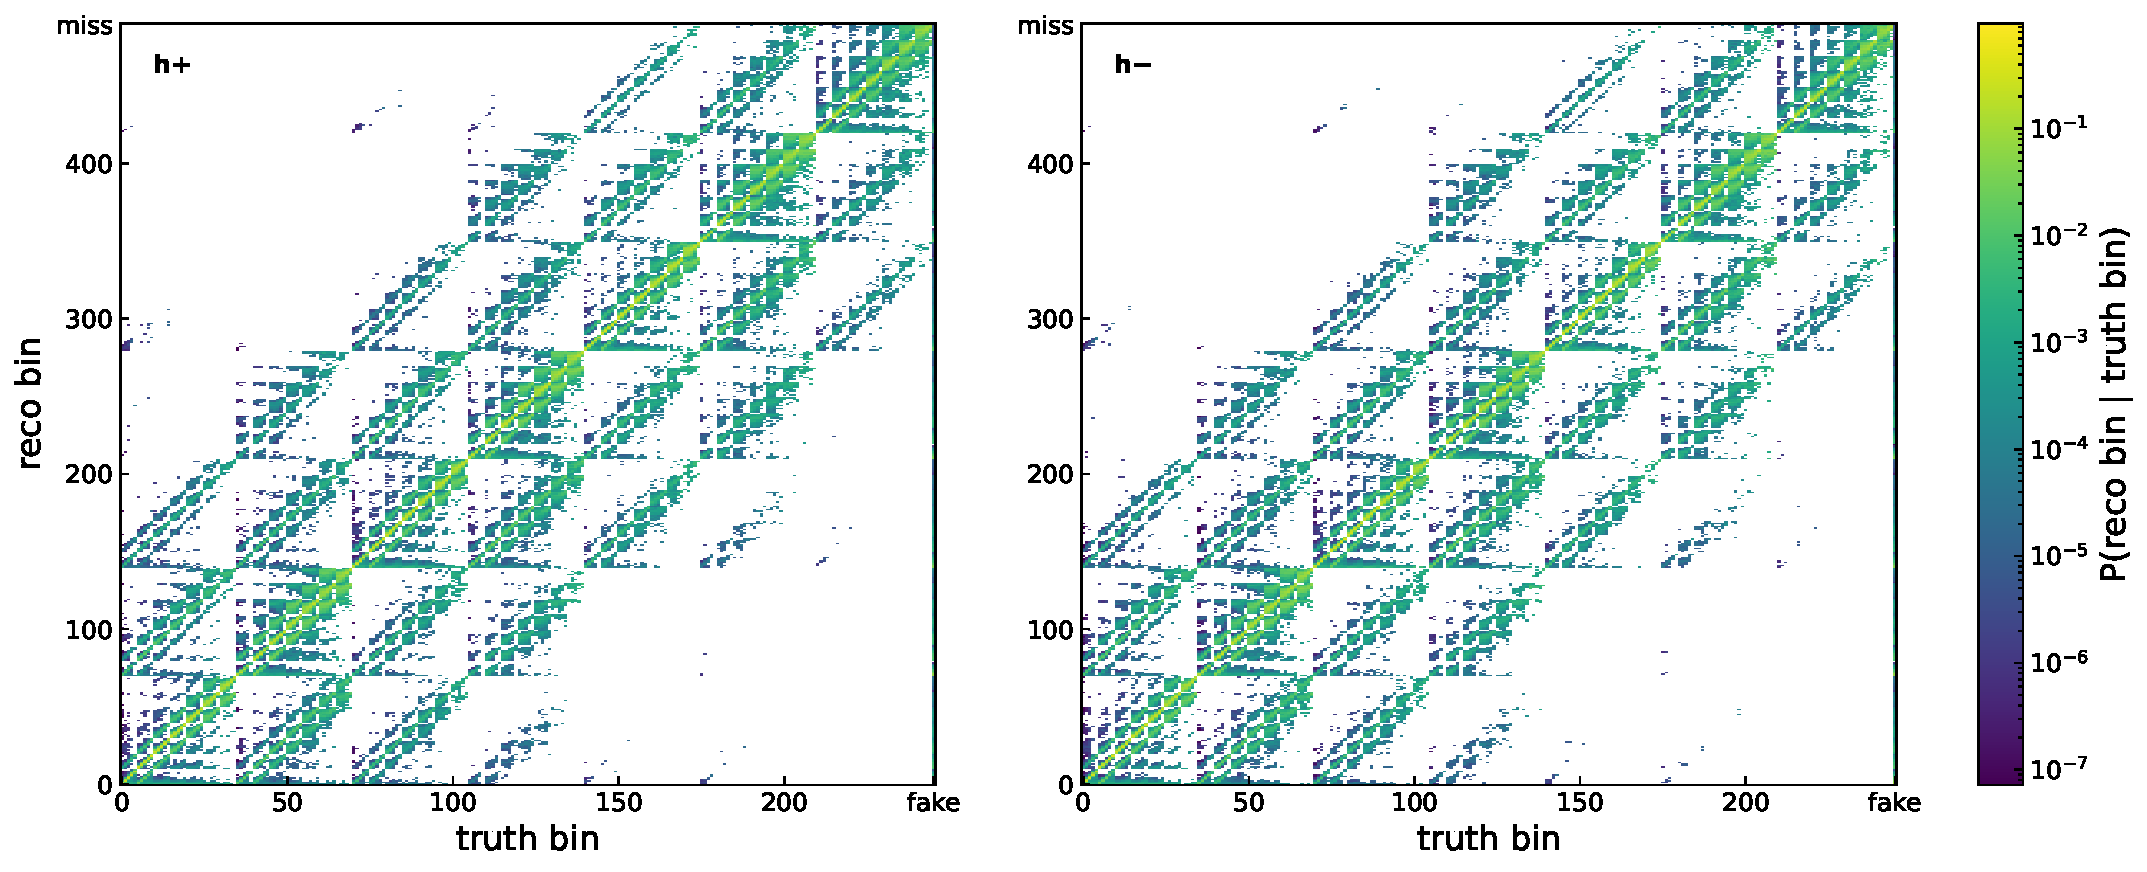
\includegraphics[width=0.92\textwidth]{figures/fig_alpha0p2_allfake_migration_matrix_z005_diagnostic_log_unstretched.pdf}
  \caption{Diagnostic/provisional all-fake migration matrix for the near-electron opening-angle veto study. The positive- and negative-charge response matrices each have shape $(491,246)$, with rows 0--489 corresponding to physical reconstructed bins, row 490 to misses, columns 0--244 to physical truth bins, and column 245 to fakes. The matrix is column-normalized as $P(\mathrm{reco\ bin}\mid\mathrm{truth\ bin})$ and displayed on a logarithmic colour scale without stretching the one-bin fake and miss extensions. Central response and release products are unchanged.}
  \label{fig:unfolding:alpha0p2-allfake-migration-matrix}
\end{figure}

\begin{figure}[t]
  \centering
  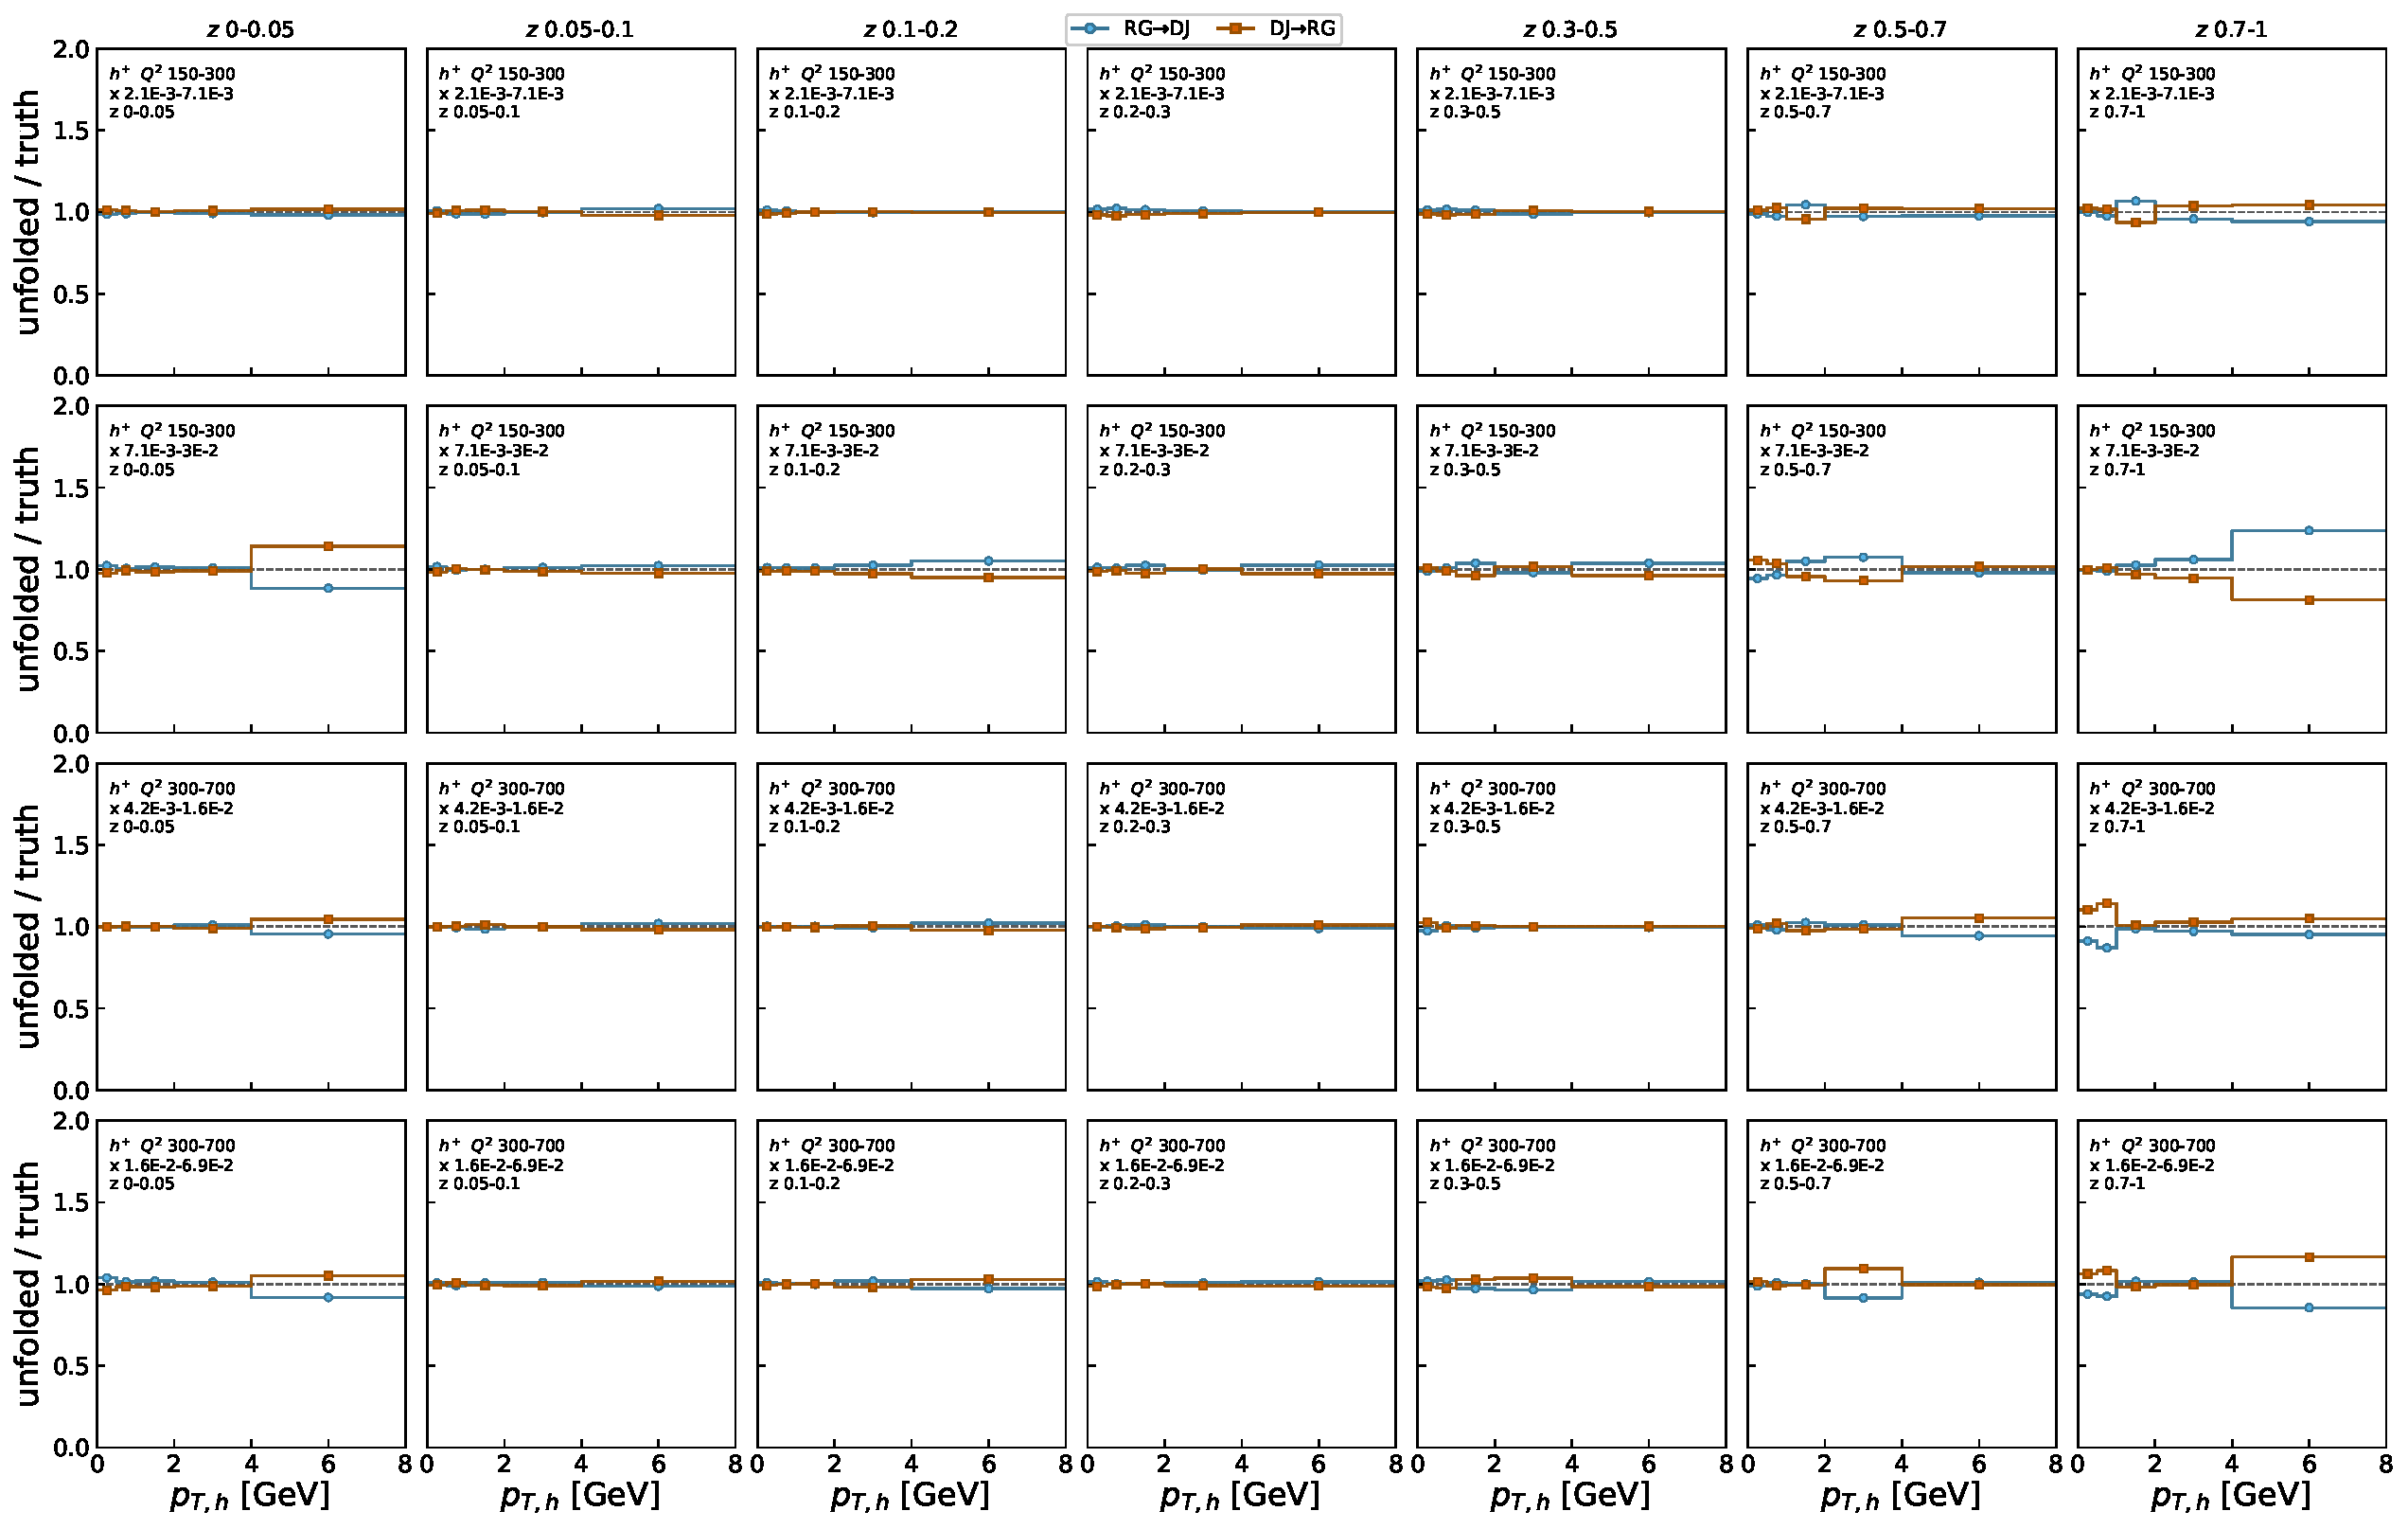
\includegraphics[width=0.92\textwidth]{figures/fig_ibu_crossclosure_7col_fullrange_z005.pdf}
  \caption{IBU cross-generator closure diagnostic in the canonical seven-column $\pTh$ layout, shown over the full ratio range 0--2. The plotted ratios are $\mathrm{DJ}\to\mathrm{RG}=N^{\mathrm{DJ\ reco,\ unfolded\ with\ RG\ response}}/N^{\mathrm{DJ\ truth}}$ and $\mathrm{RG}\to\mathrm{DJ}=N^{\mathrm{RG\ reco,\ unfolded\ with\ DJ\ response}}/N^{\mathrm{RG\ truth}}$. This is a cross-generator closure check only; no self-closure is included.}
  \label{fig:unfolding:ibu-crossclosure-fullrange}
\end{figure}

\begin{figure}[t]
  \centering
  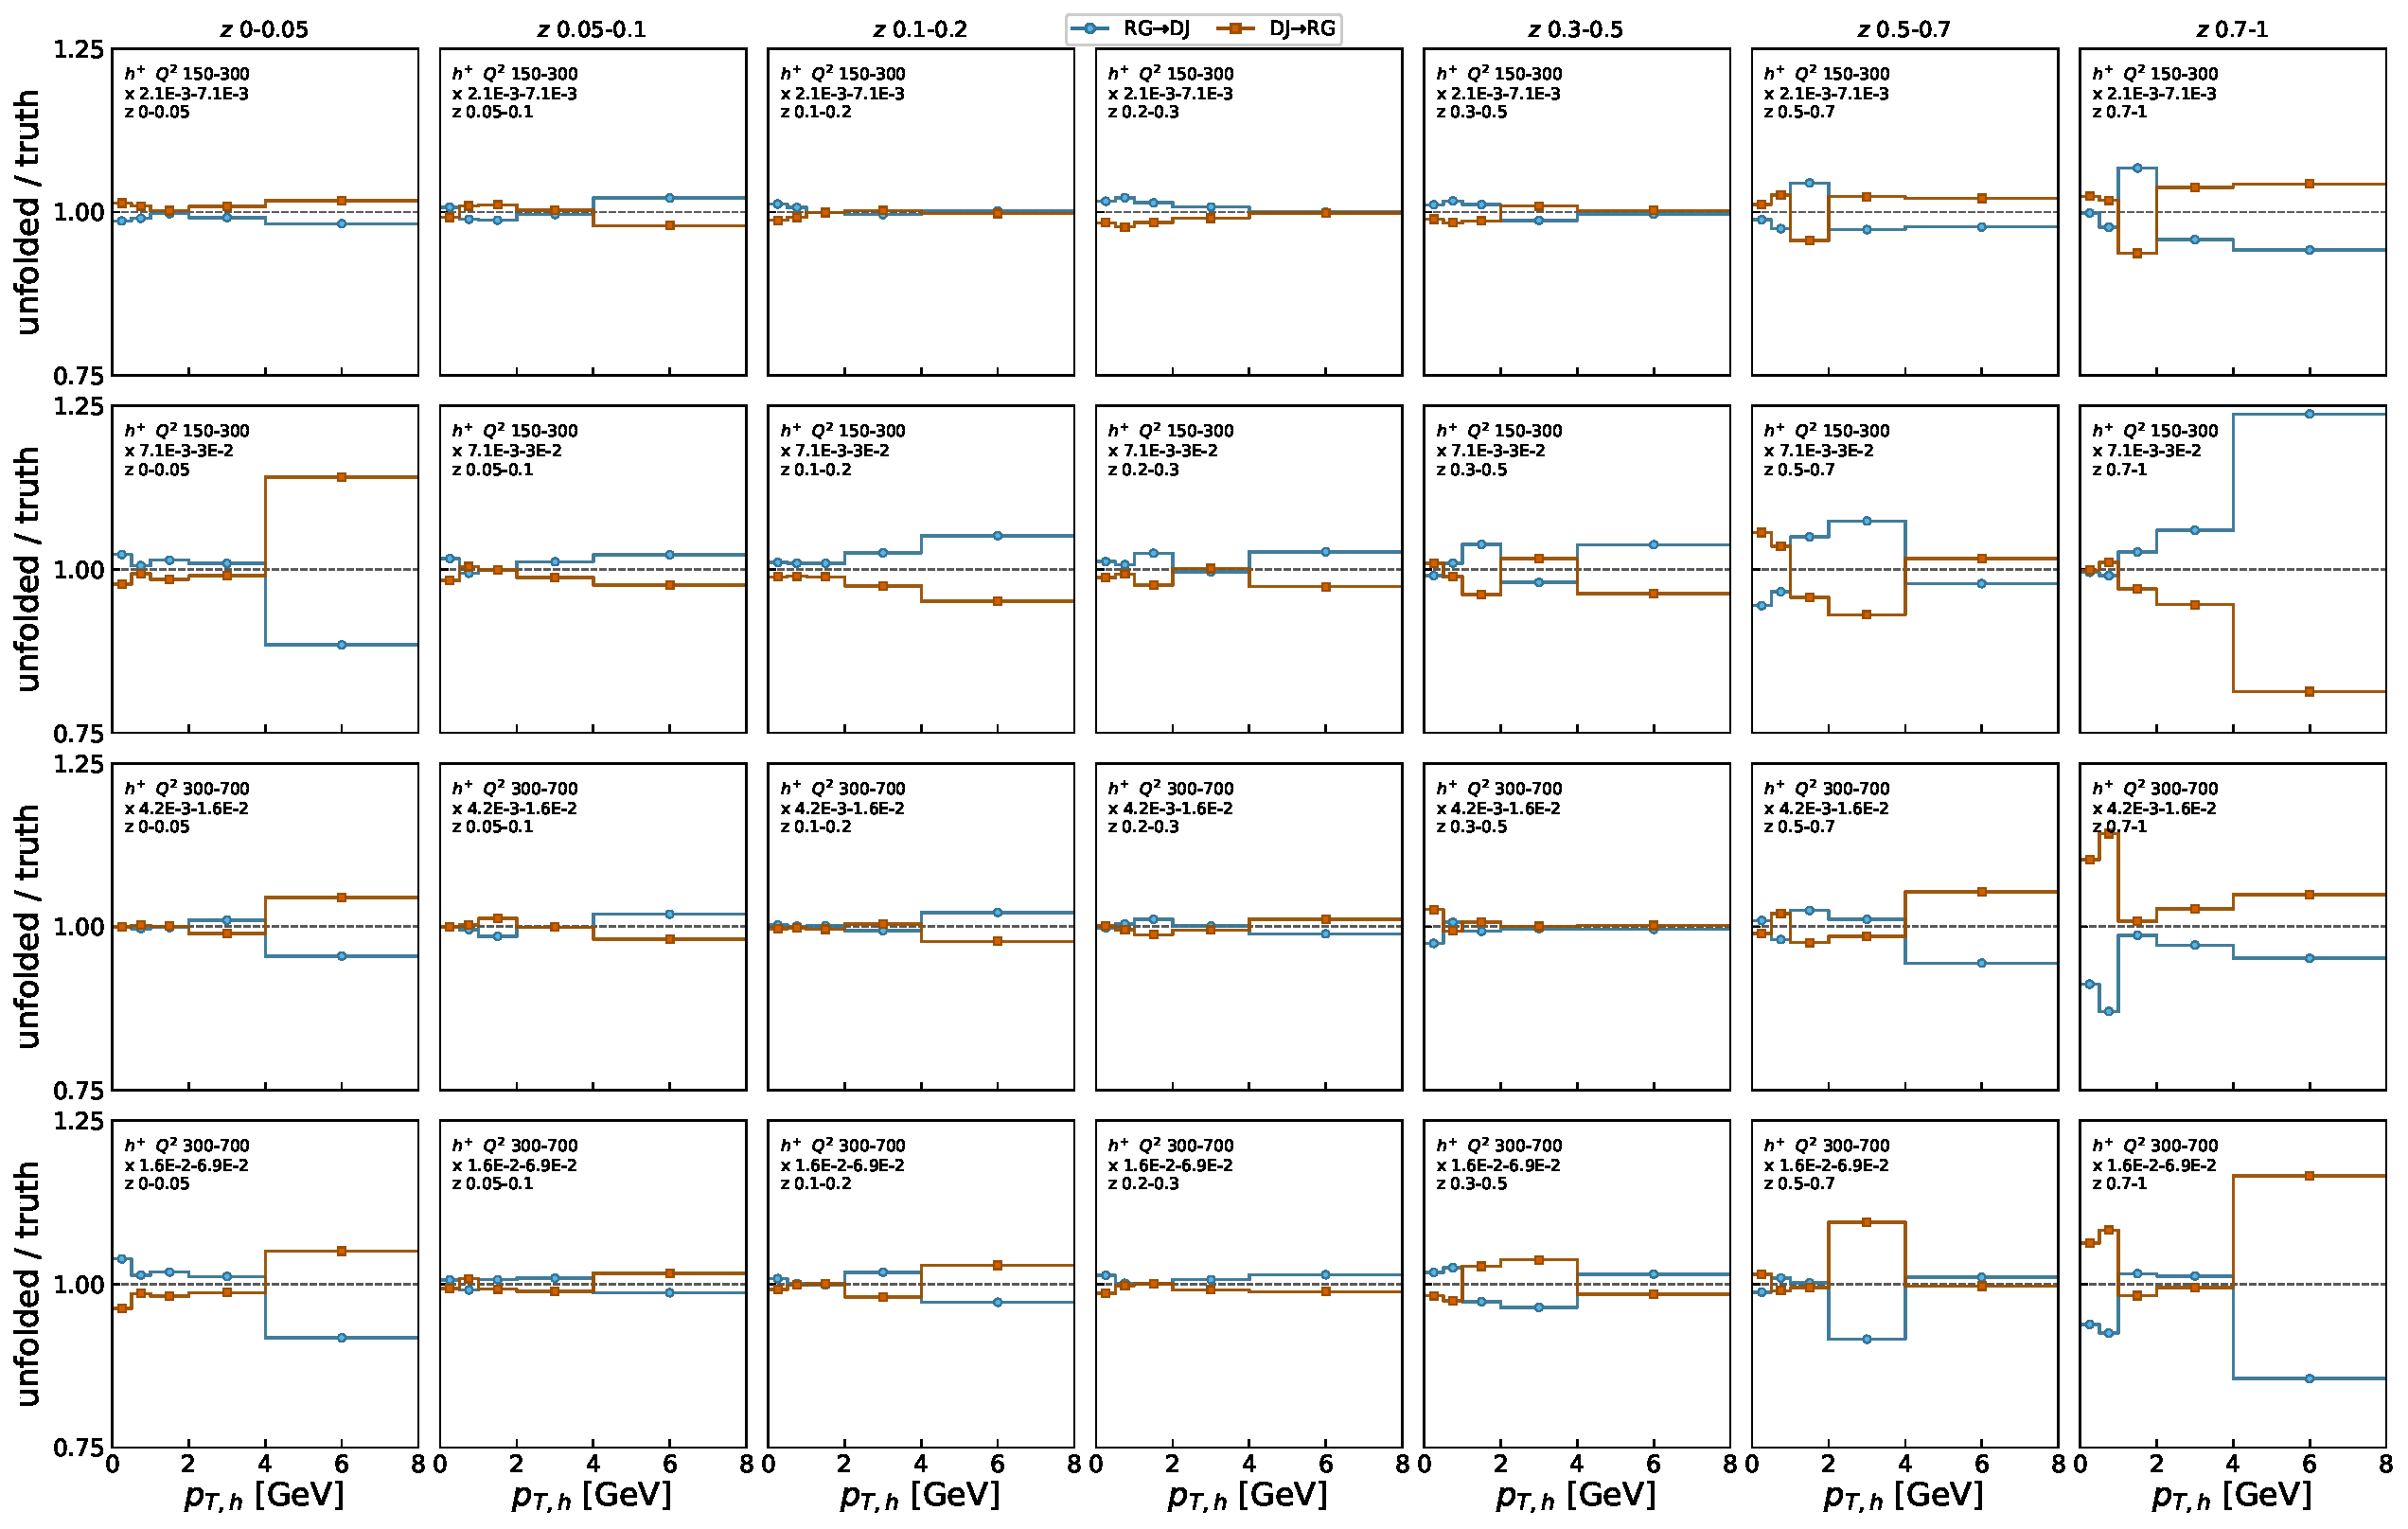
\includegraphics[width=0.92\textwidth]{figures/fig_ibu_crossclosure_7col_zoom_z005.pdf}
  \caption{Zoomed IBU cross-generator closure diagnostic in the canonical seven-column $\pTh$ layout, displaying the ratio range 0.75--1.25. Ratio definitions are the same as in Fig.~\ref{fig:unfolding:ibu-crossclosure-fullrange}; the diagnostic is cross-generator only and includes no self-closure component.}
  \label{fig:unfolding:ibu-crossclosure-zoom}
\end{figure}

\begin{figure}[t]
  \centering
  \begin{subfigure}[t]{0.95\textwidth}
    \centering
    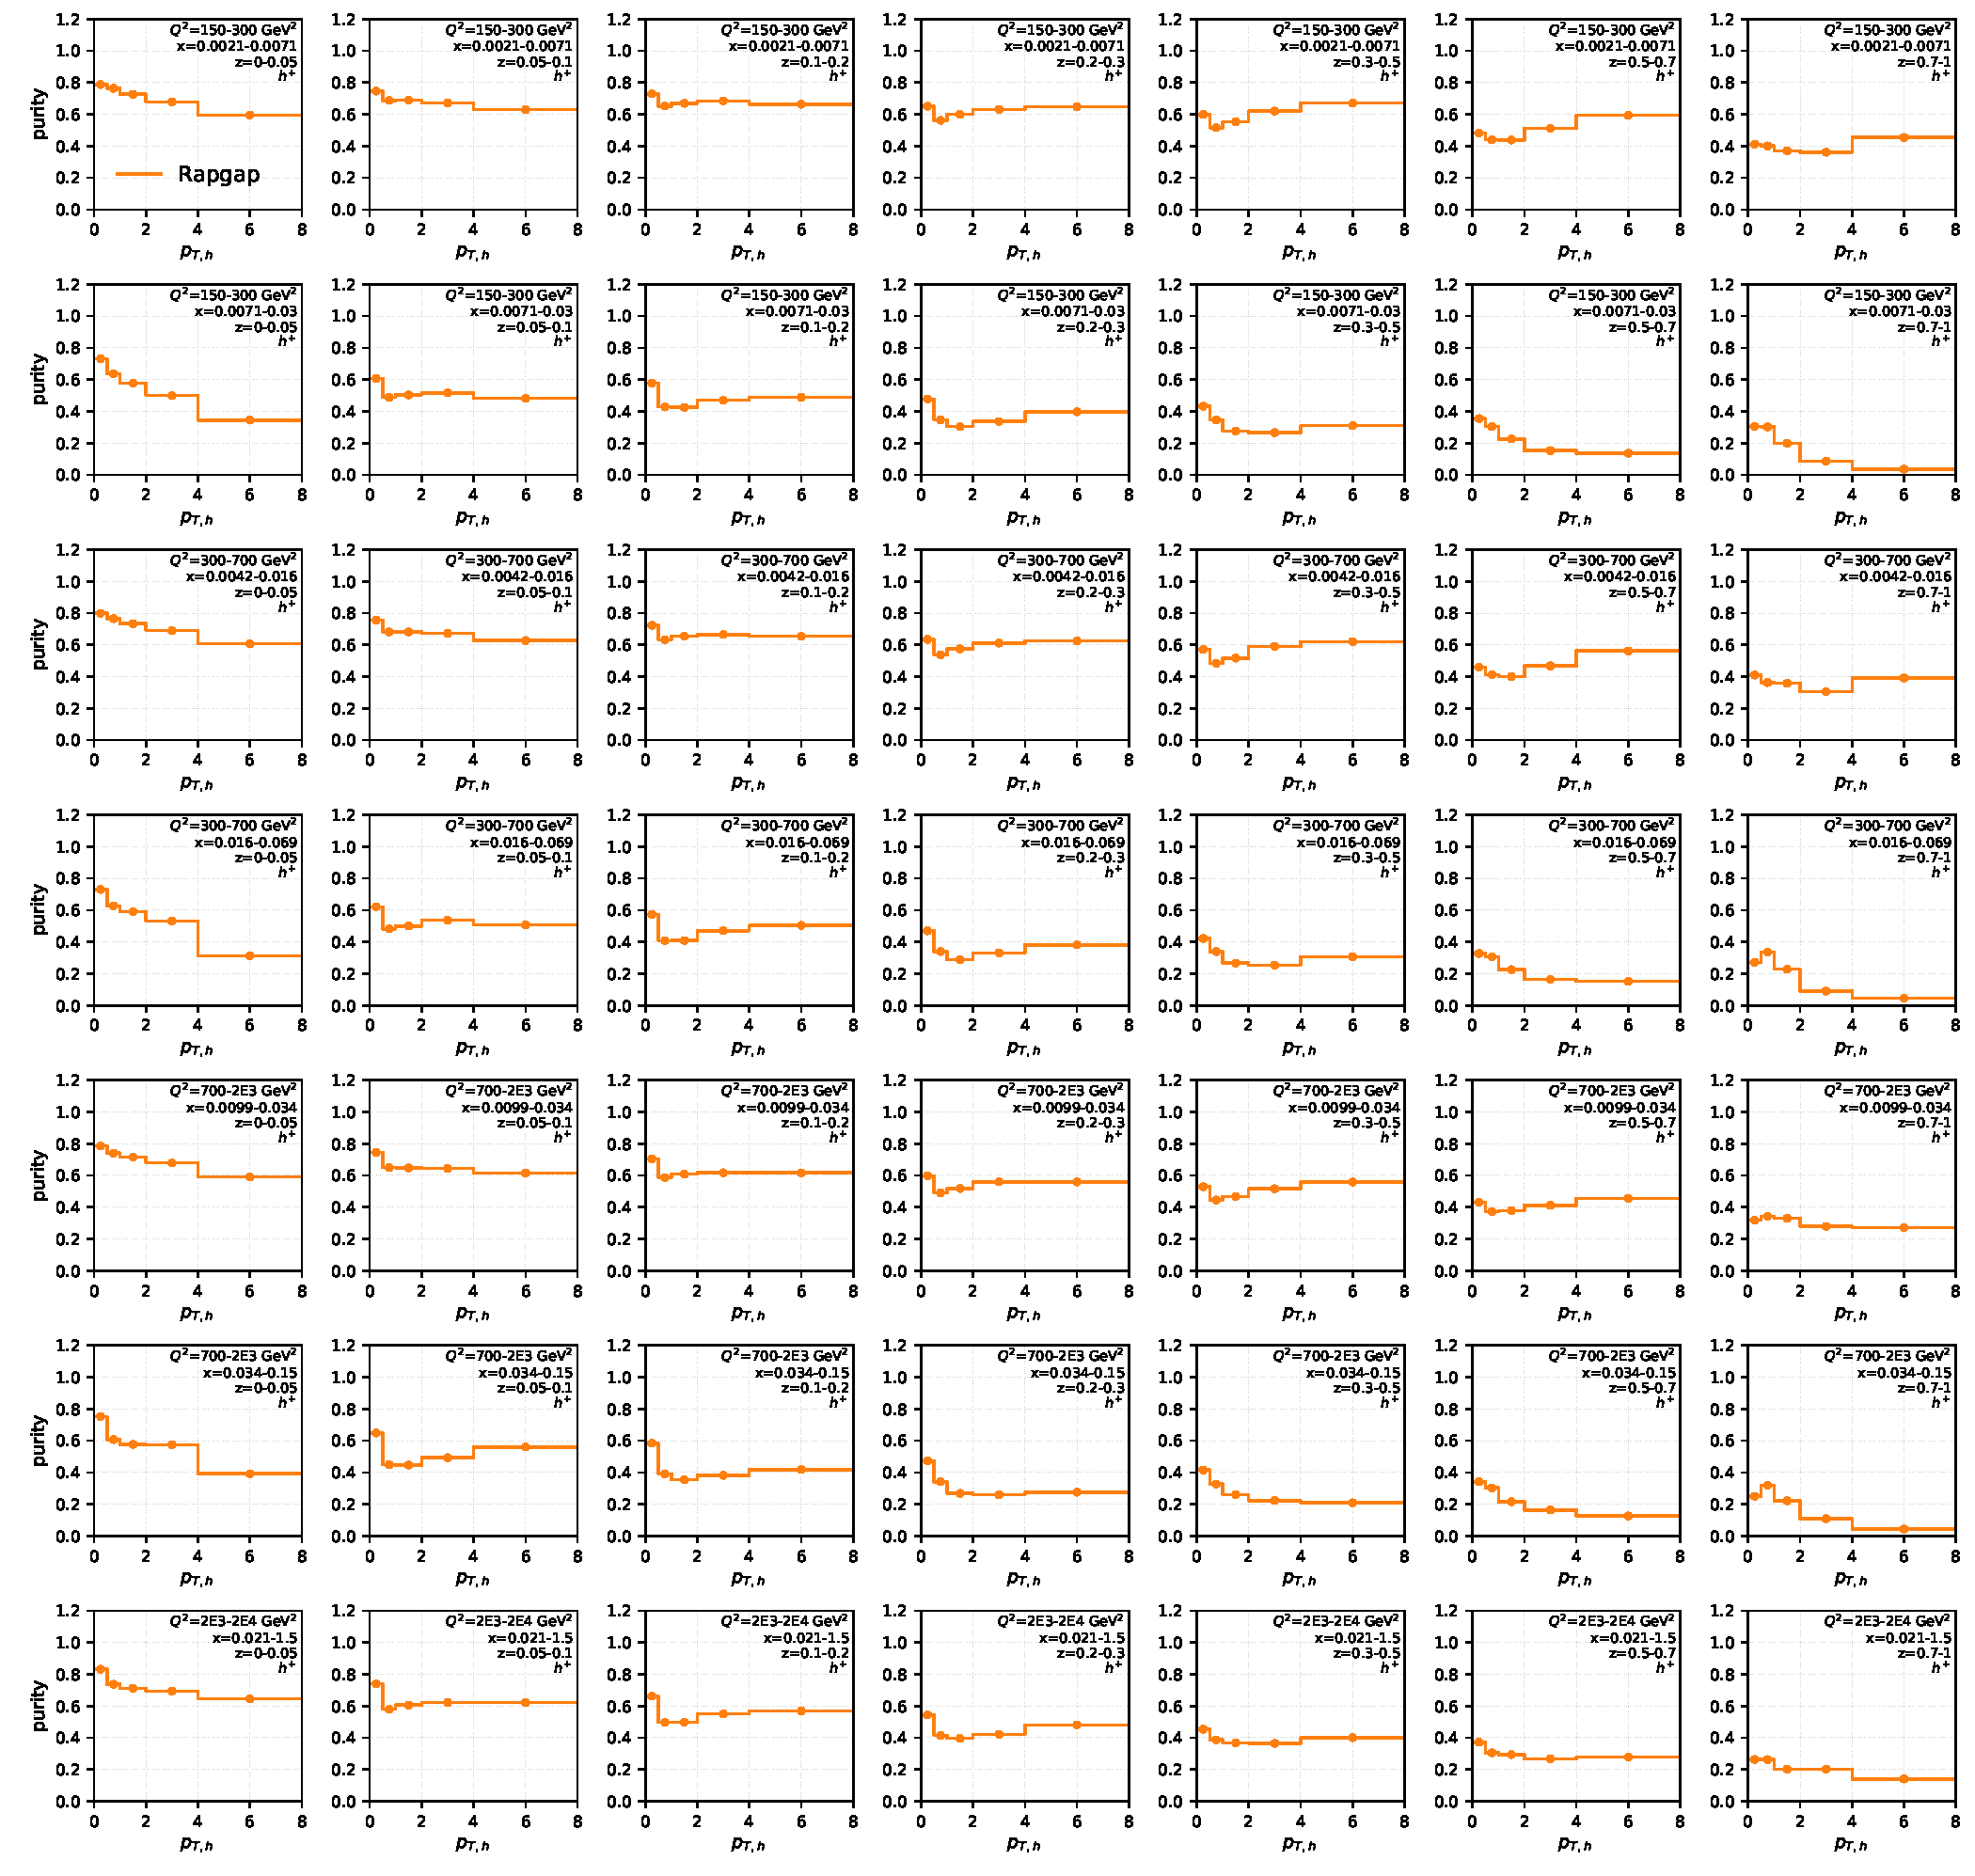
\includegraphics[width=\textwidth]{figures/fig_response_purity_hp_7col_20261007.pdf}
    \caption{Purity versus $\pTh$ for $\hplus$ in all bins, with the fake column included in $N_{\mathrm{rec}}$.}
  \end{subfigure}
  \hfill
  \begin{subfigure}[t]{0.95\textwidth}
    \centering
    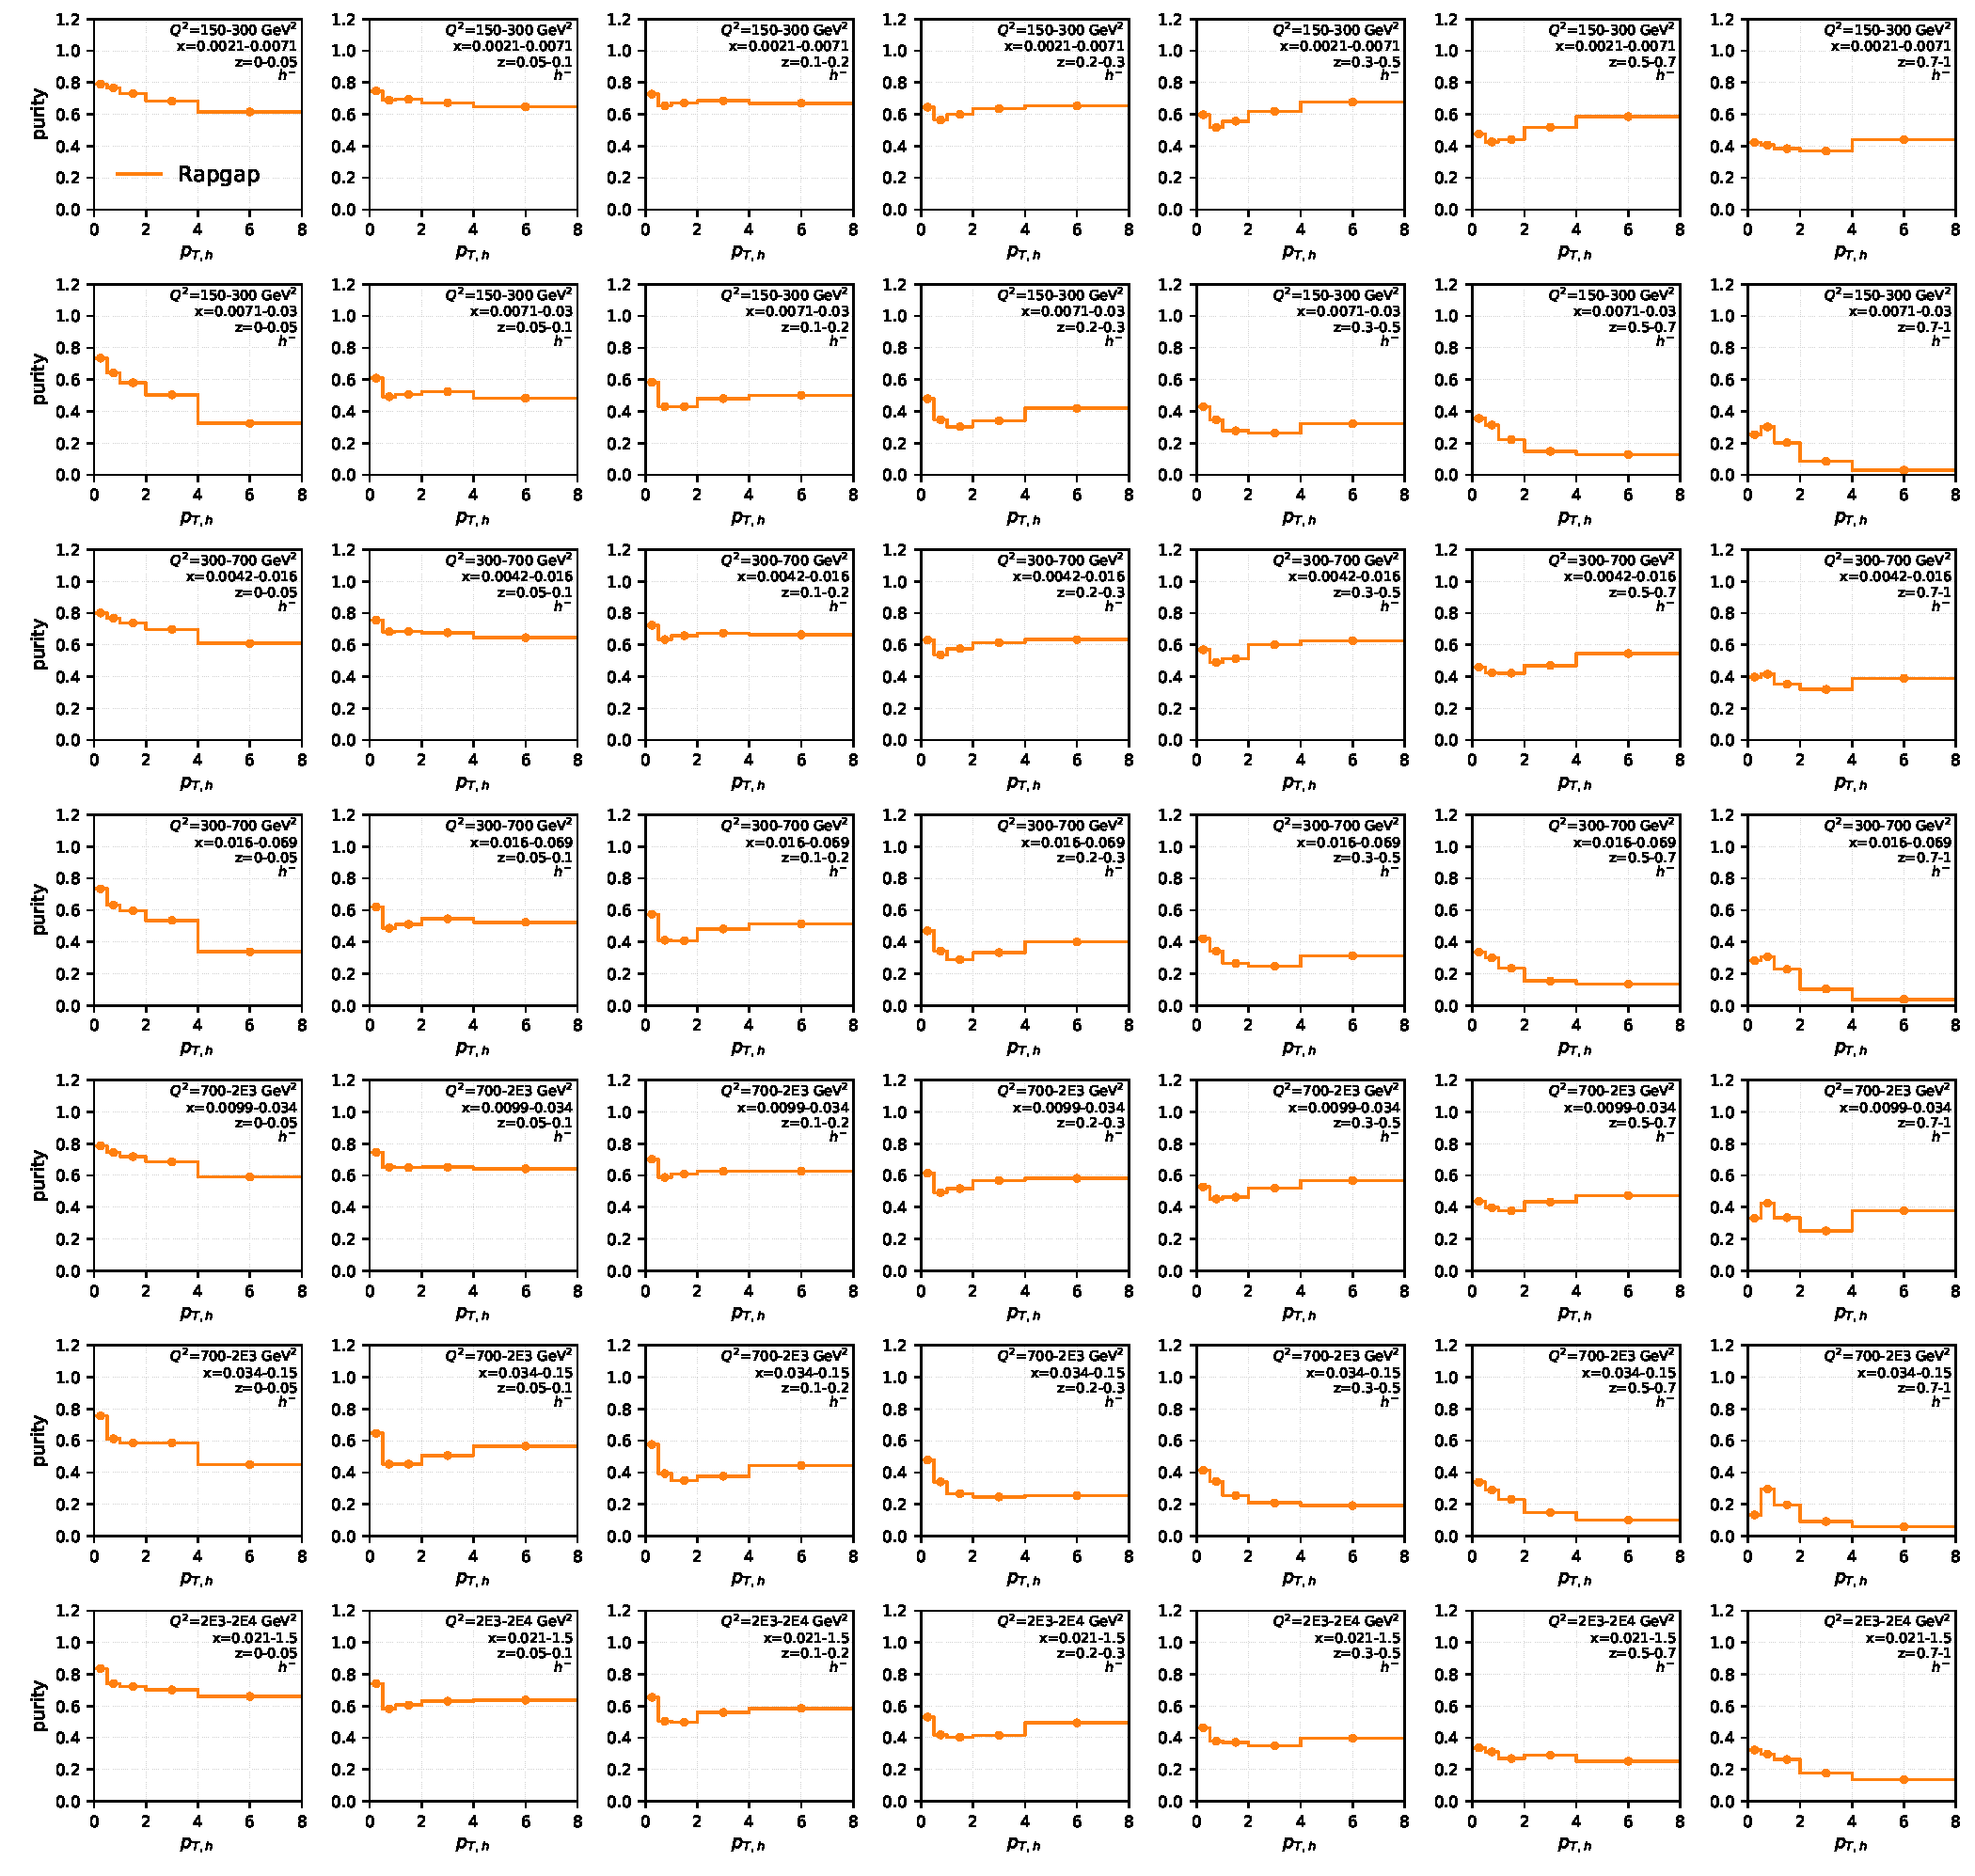
\includegraphics[width=\textwidth]{figures/fig_response_purity_hm_7col_20261007.pdf}
    \caption{$\hminus$, with the fake column included in $N_{\mathrm{rec}}$.}
    \label{fig:unfolding:alpha0p2-purity-hm}
  \end{subfigure}
  \caption{Purity versus $\pTh$ for $\hplus$ and $\hminus$ in all bins. The denominator $N_{\mathrm{rec}}$ includes the fake column.}
  \label{fig:unfolding:alpha0p2-purity}
\end{figure}

\begin{figure}[t]
  \centering
  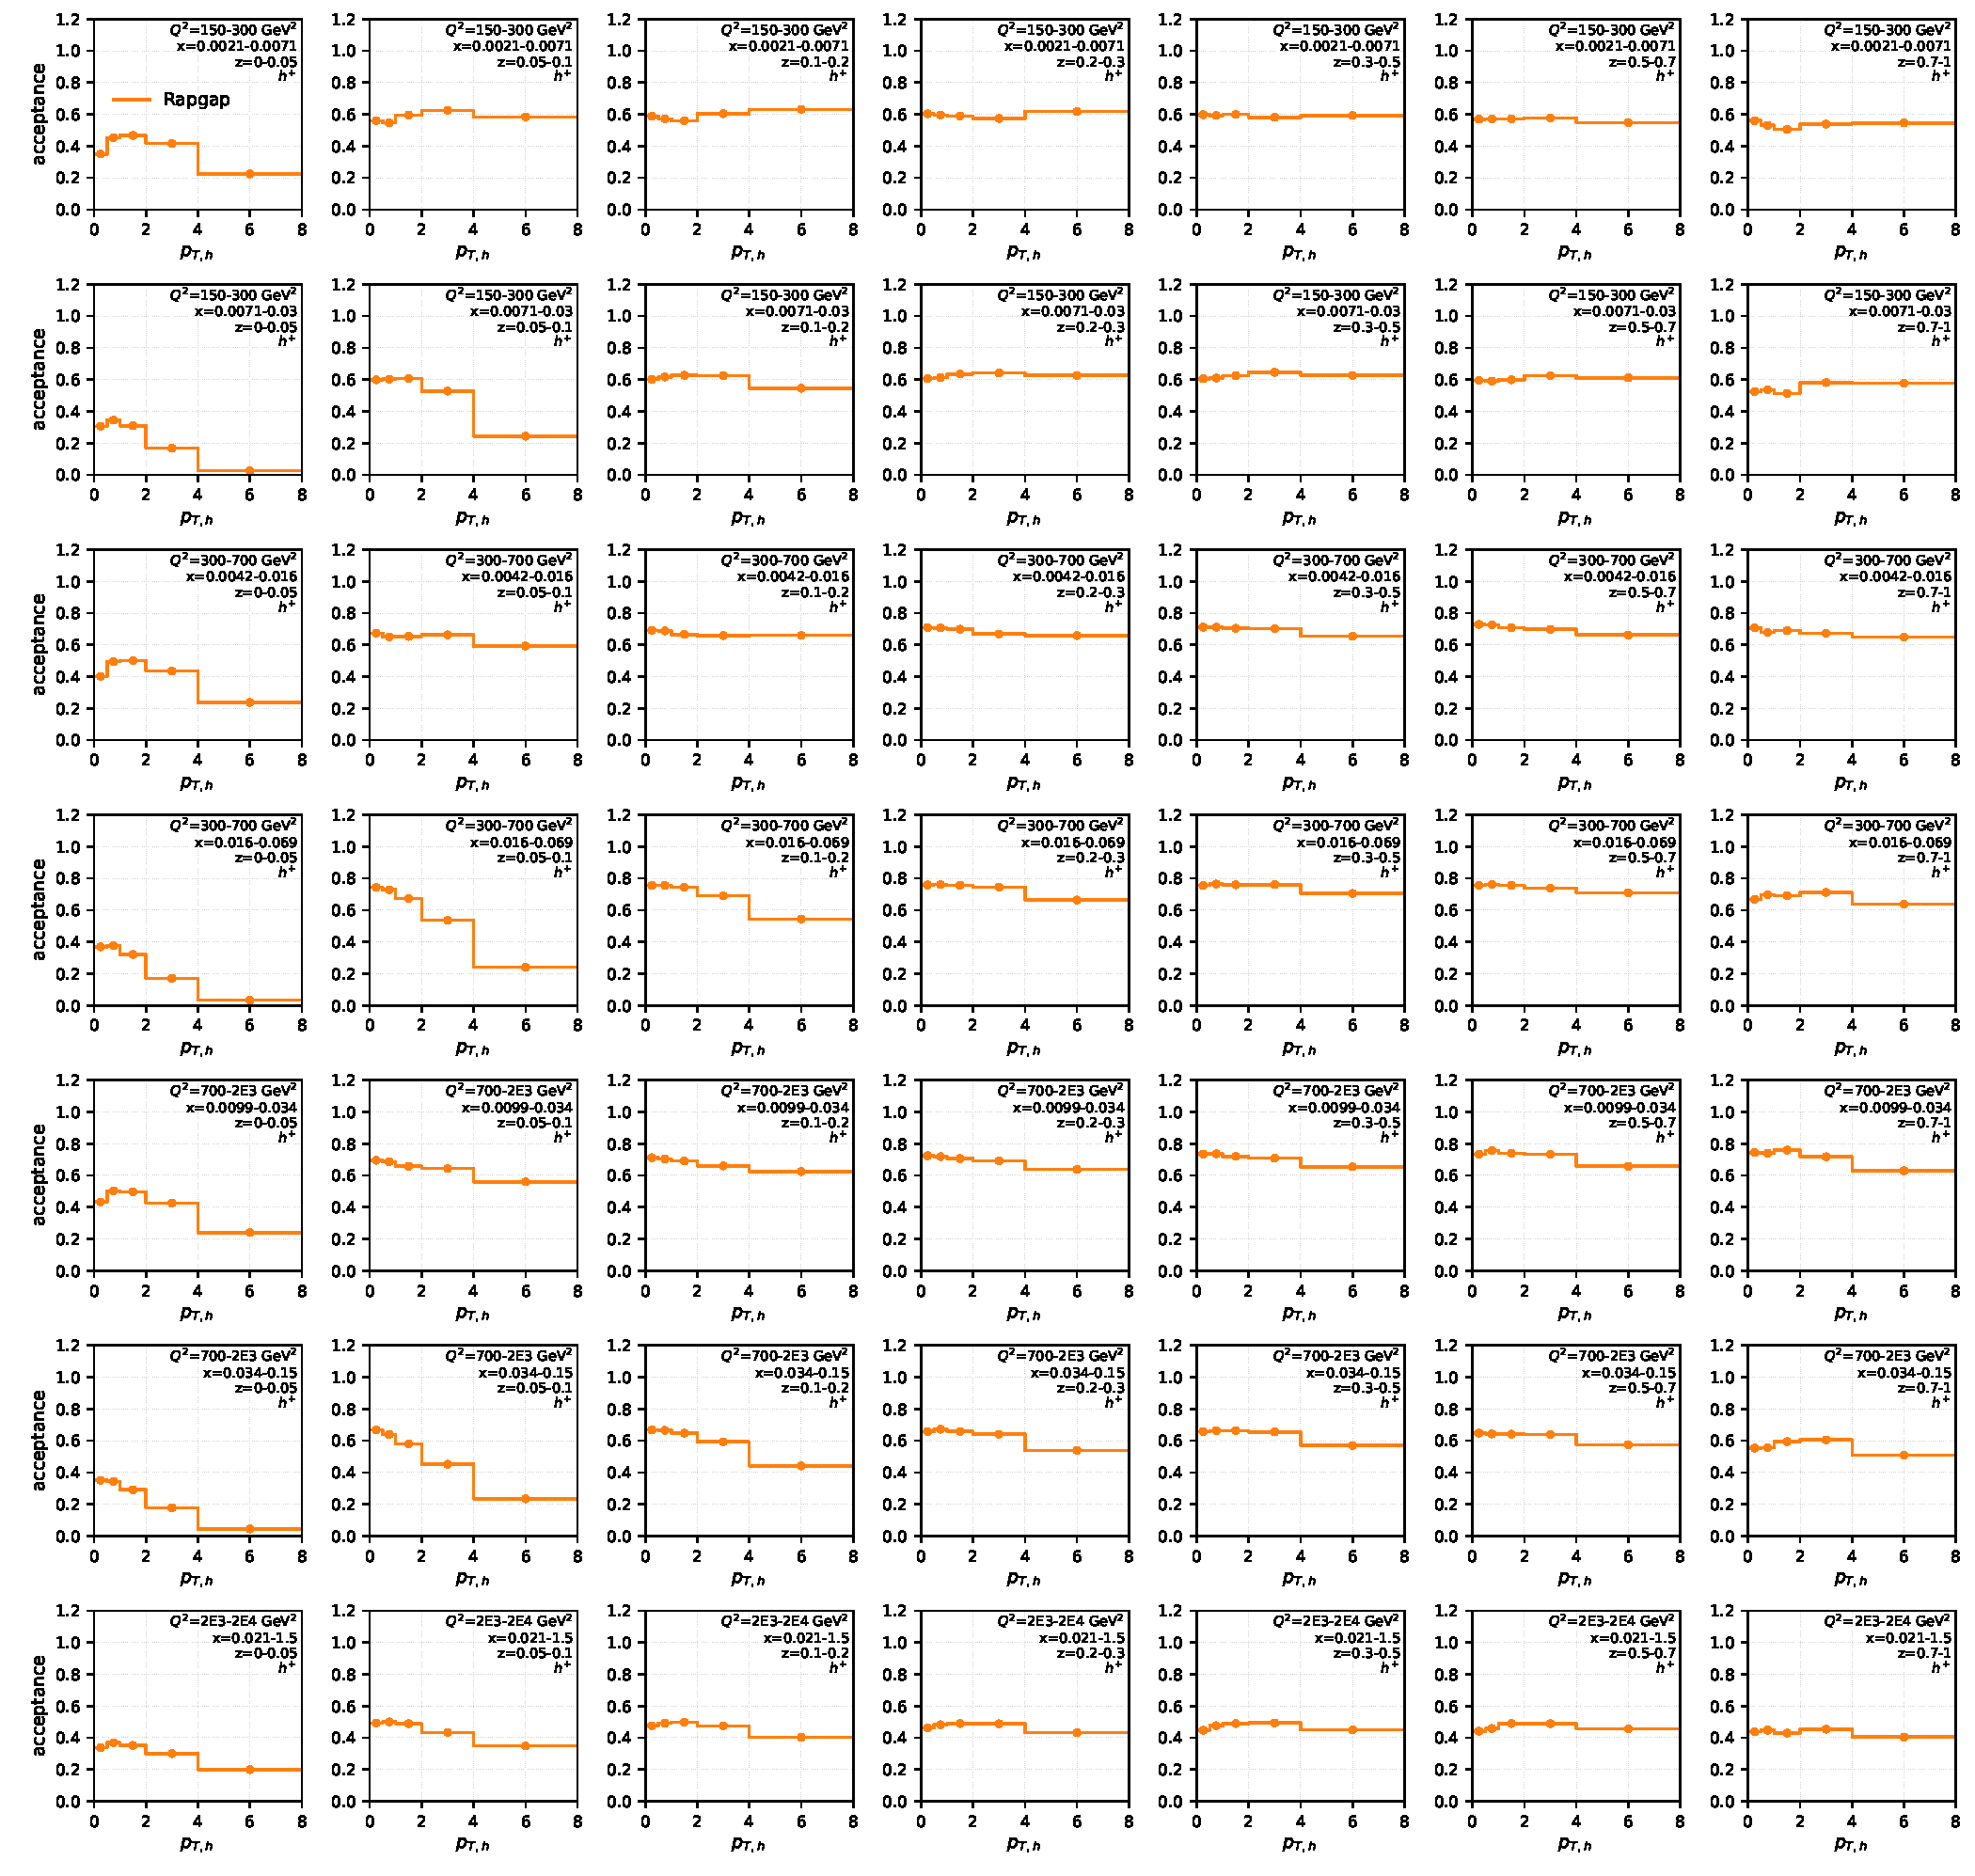
\includegraphics[width=0.92\textwidth]{figures/fig_response_acceptance_hp_7col_20261007.pdf}
  \caption{Acceptance versus $\pTh$ for $\hplus$ in all bins.}
  \label{fig:unfolding:alpha0p2-acceptance-hp}
\end{figure}

\begin{figure}[t]
  \centering
  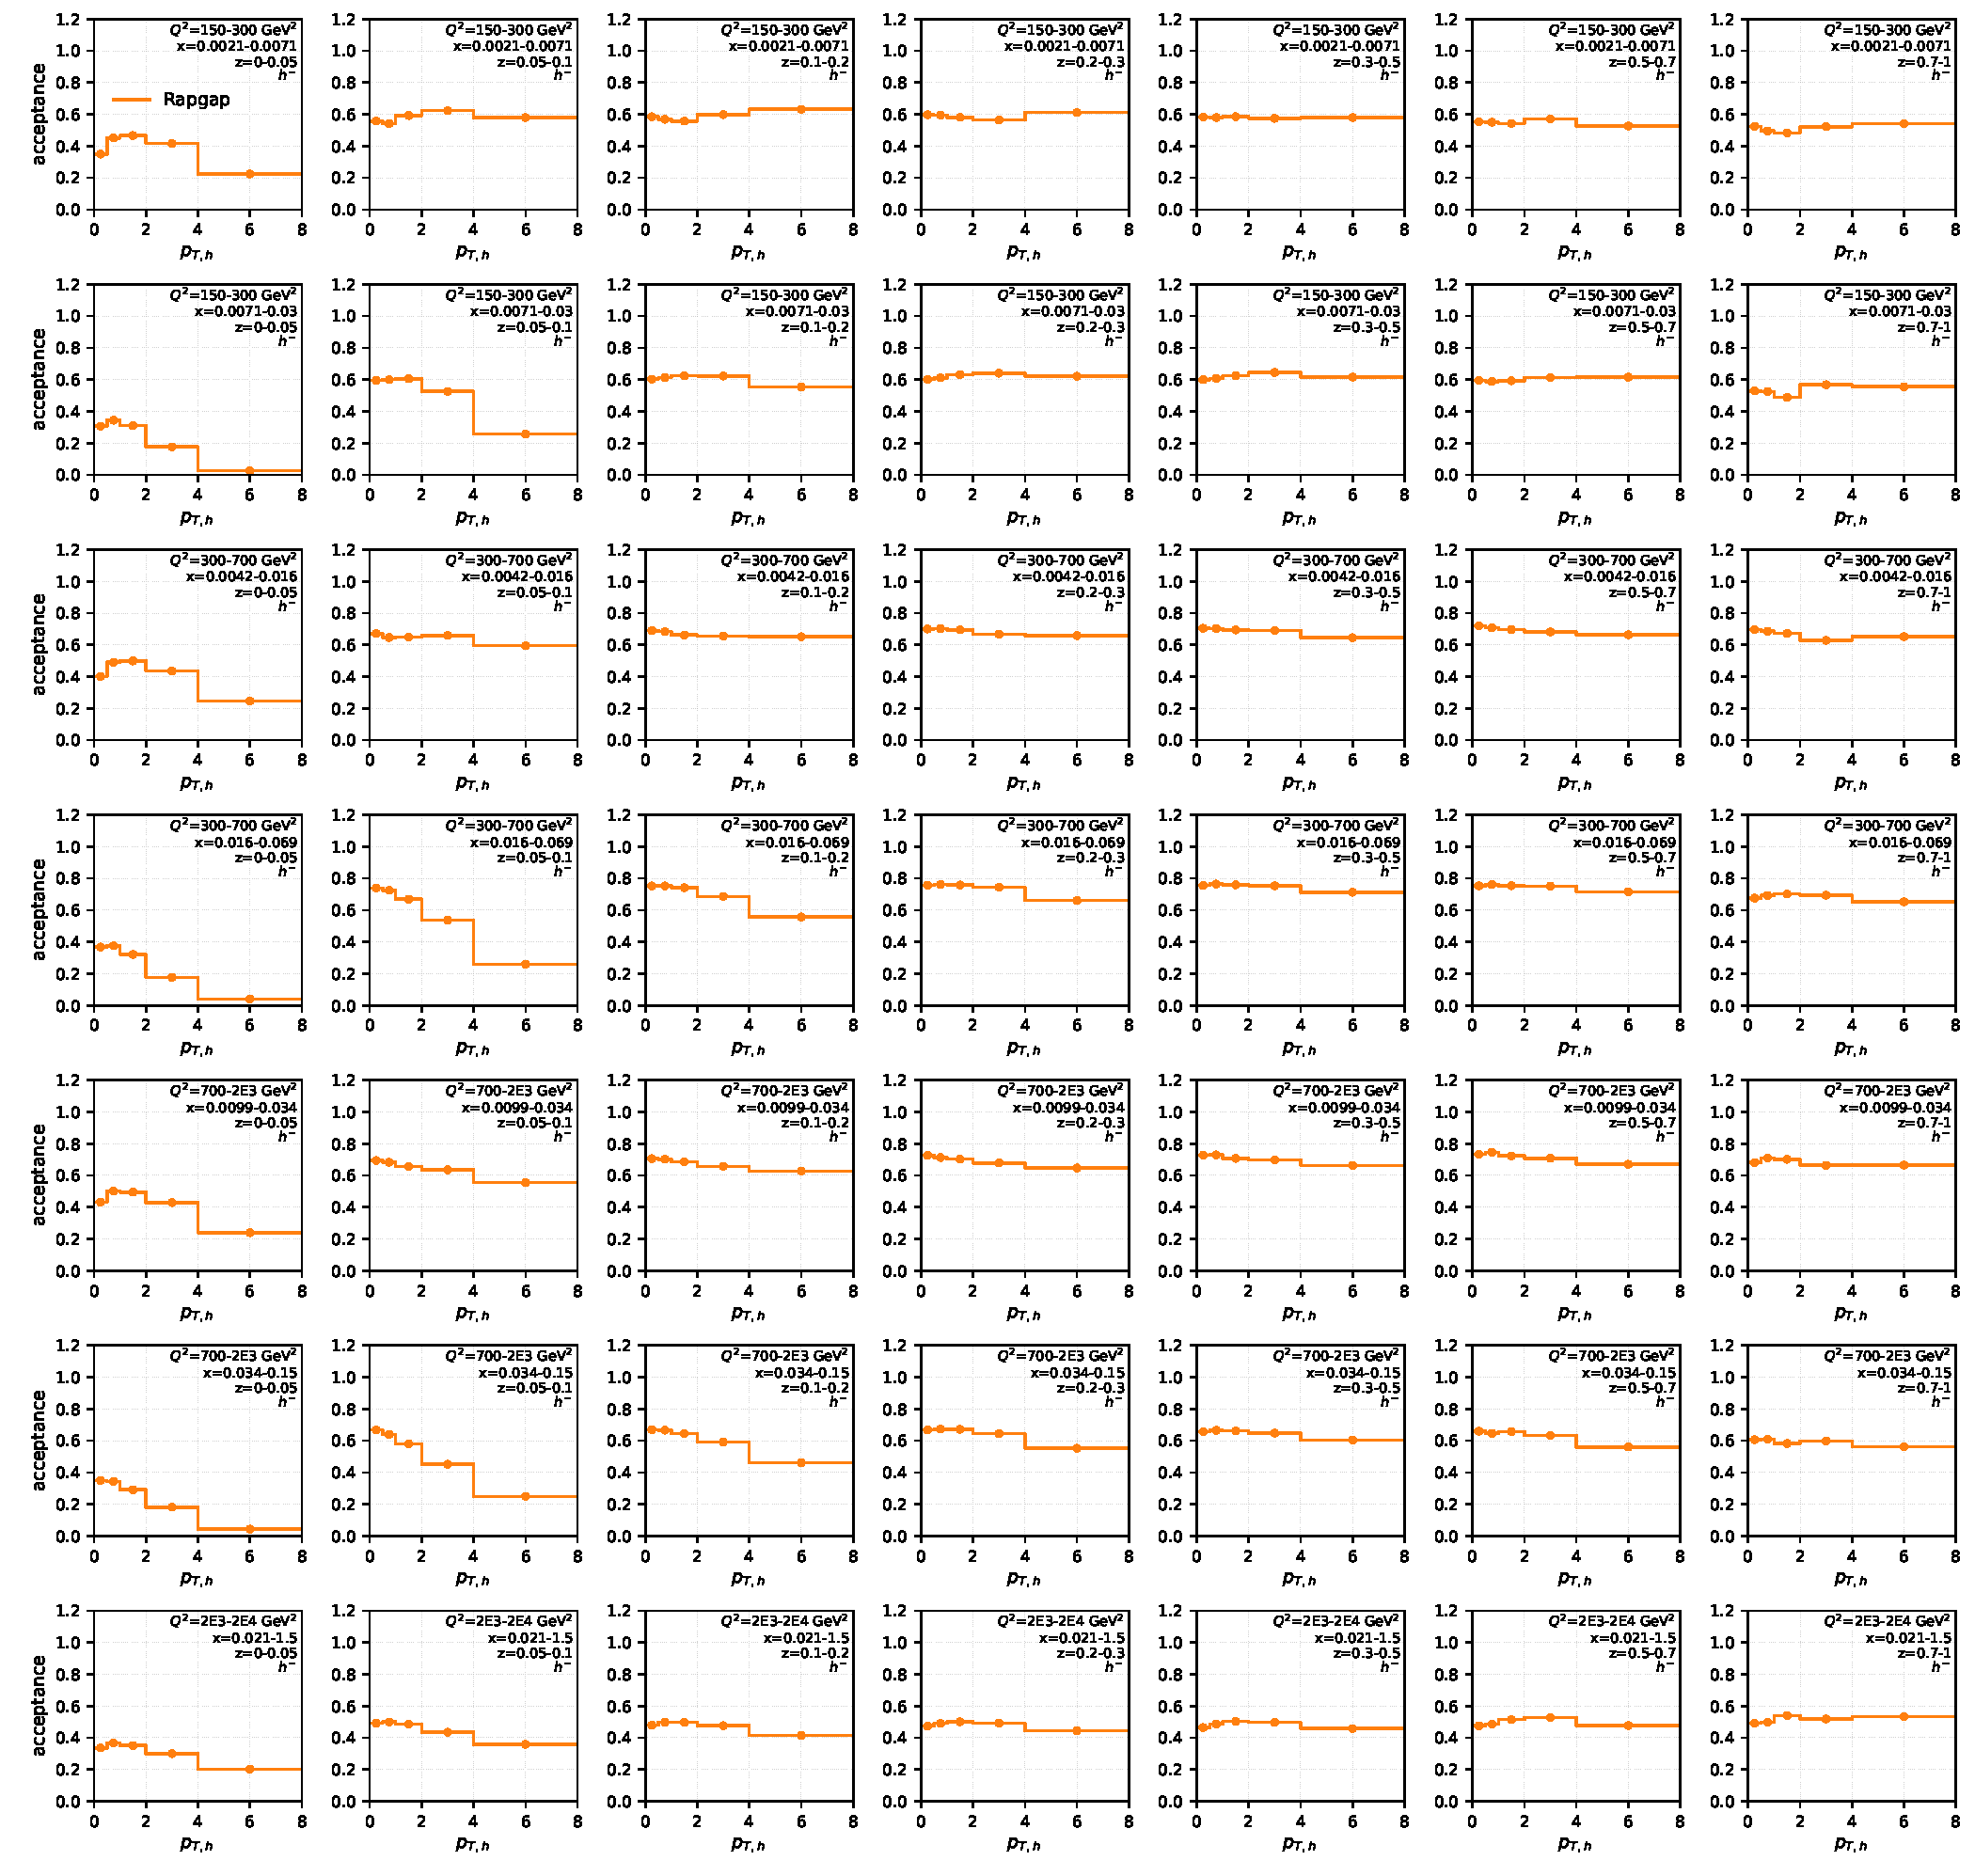
\includegraphics[width=0.92\textwidth]{figures/fig_response_acceptance_hm_7col_20261007.pdf}
  \caption{Acceptance versus $\pTh$ for $\hminus$ in all bins.}
  \label{fig:unfolding:alpha0p2-acceptance-hm}
\end{figure}

\subsection{Cross-check with TUnfold}
\label{sec:unfolding:tunfold-crosscheck}

Native ROOT/TUnfold v6 is retained as the validated second-method cross-check.  The iterative Bayesian unfolding, with the response's own generator-level prior and four iterations, is the final nominal method; the TUnfold result is diagnostic only.  The comparison uses the earlier detector-interaction-corrected basis without the electron cone, at raw level, which is also the basis of the existing figures in this section.  This superseded observable basis is retained for the diagnostic comparison; regeneration on the current basis is a separate pending item.

For TUnfold, $\tau=10^{-5}$ was selected with a 1\%-absolute-bias gate on both generator chains.  The delivered solution is $\max(x,0)$; its one-sided clipping bias, $+0.028\%$ for $h^+$ and $+0.0107\%$ for $h^-$, is accounted for separately.  In a 1000-toy validation on identical toys, both methods were unbiased and the TUnfold statistical uncertainty was toy-validated, with toy-to-reported ratios of 0.975 and 0.969 for $h^+$ and $h^-$, respectively.  TUnfoldSys covariance-in-solve propagation gave total-full median uncertainties of 9.16\% and 10.10\%, compared with 8.19\% and 8.41\% in the release budget, with the excess attributed in the validation record.  The method-choice record is documented in \texttt{docs/unfolding/pmethod\_decision\_dossier\_2026-10-14.md}.

\begin{figure}[t]
  \centering
  \begin{subfigure}[t]{0.49\textwidth}
    \centering
    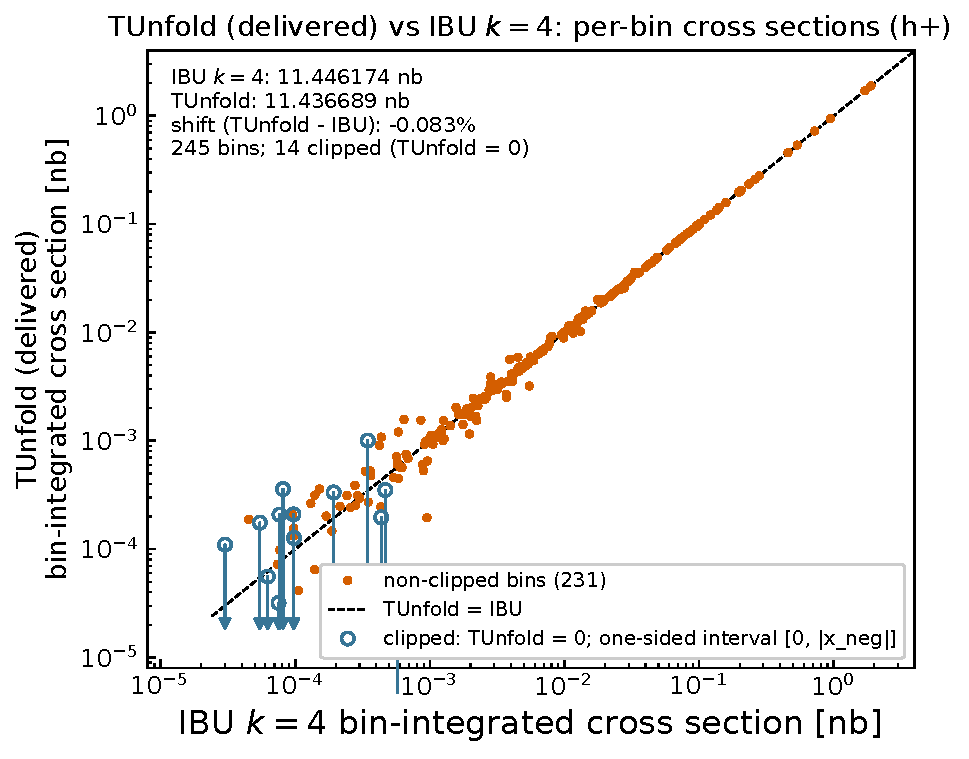
\includegraphics[width=\textwidth]{figures/fig_unfolding_tunfold_vs_ibu_scatter_z005_hplus.pdf}
    \caption{$\hplus$.}
  \end{subfigure}
  \hfill
  \begin{subfigure}[t]{0.49\textwidth}
    \centering
    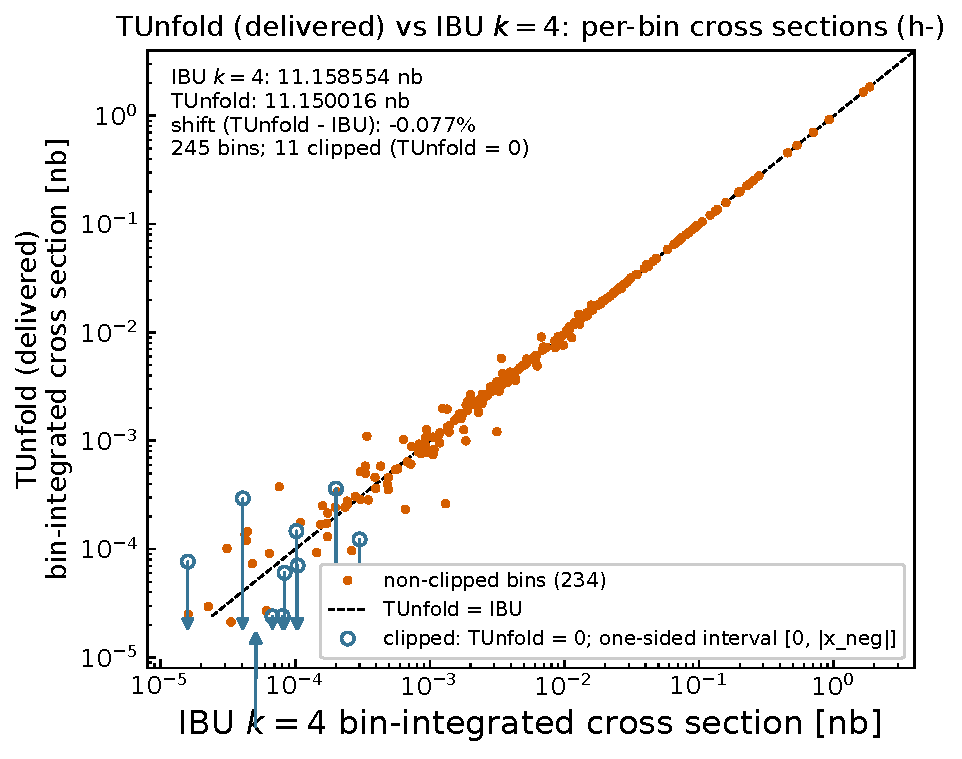
\includegraphics[width=\textwidth]{figures/fig_unfolding_tunfold_vs_ibu_scatter_z005_hminus.pdf}
    \caption{$\hminus$.}
  \end{subfigure}
  \caption{Per-bin logarithmic scatter comparison of the delivered TUnfold result with the nominal iterative Bayesian unfolding; the diagonal denotes equality.  These raw-level diagnostics use the superseded detector-interaction-corrected basis without the electron cone.  TUnfold uses $\tau=10^{-5}$ and delivers $\max(x,0)$: bins clipped from negative TUnfold values are shown as open markers at the one-sided upper value with limit-style arrows.  The comparison is retained as a diagnostic cross-check; the iterative Bayesian unfolding is nominal.}
  \label{fig:unfolding:tunfold-vs-ibu-scatter}
\end{figure}

\begin{figure}[t]
  \centering
  \begin{subfigure}[t]{0.49\textwidth}
    \centering
    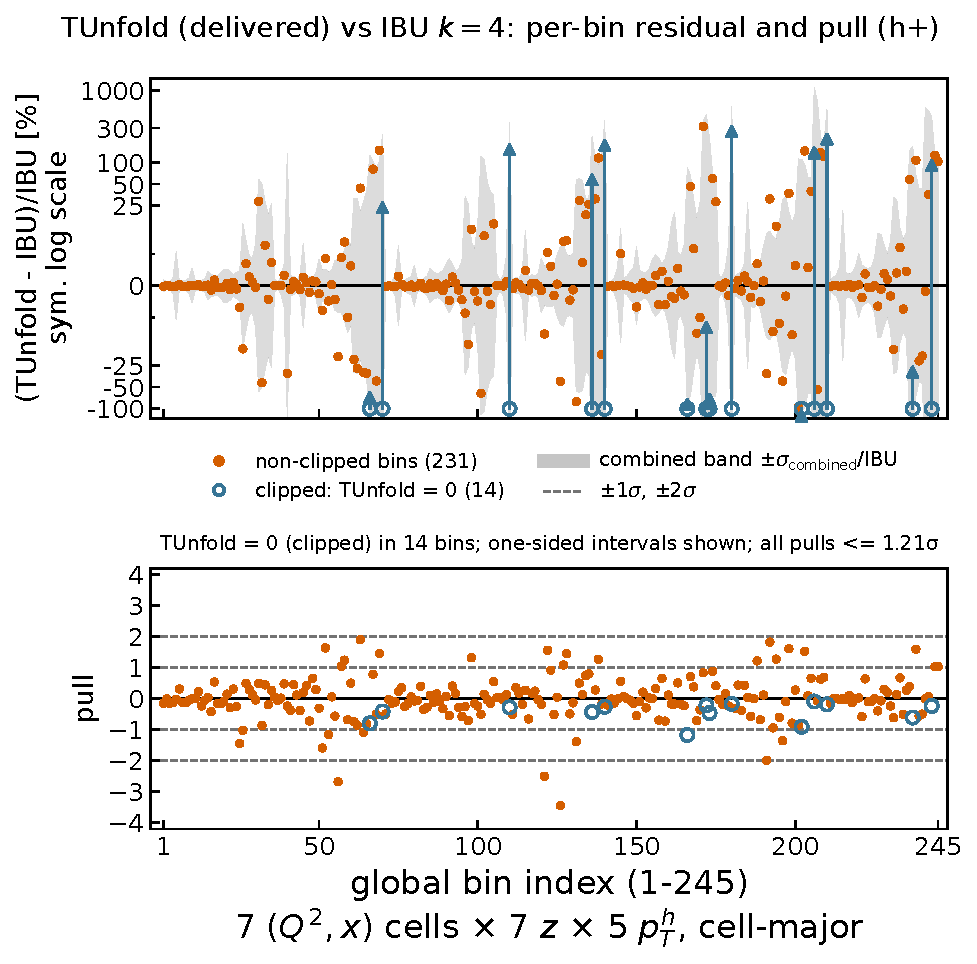
\includegraphics[width=\textwidth]{figures/fig_unfolding_tunfold_vs_ibu_residualpull_z005_hplus.pdf}
    \caption{$\hplus$.}
  \end{subfigure}
  \hfill
  \begin{subfigure}[t]{0.49\textwidth}
    \centering
    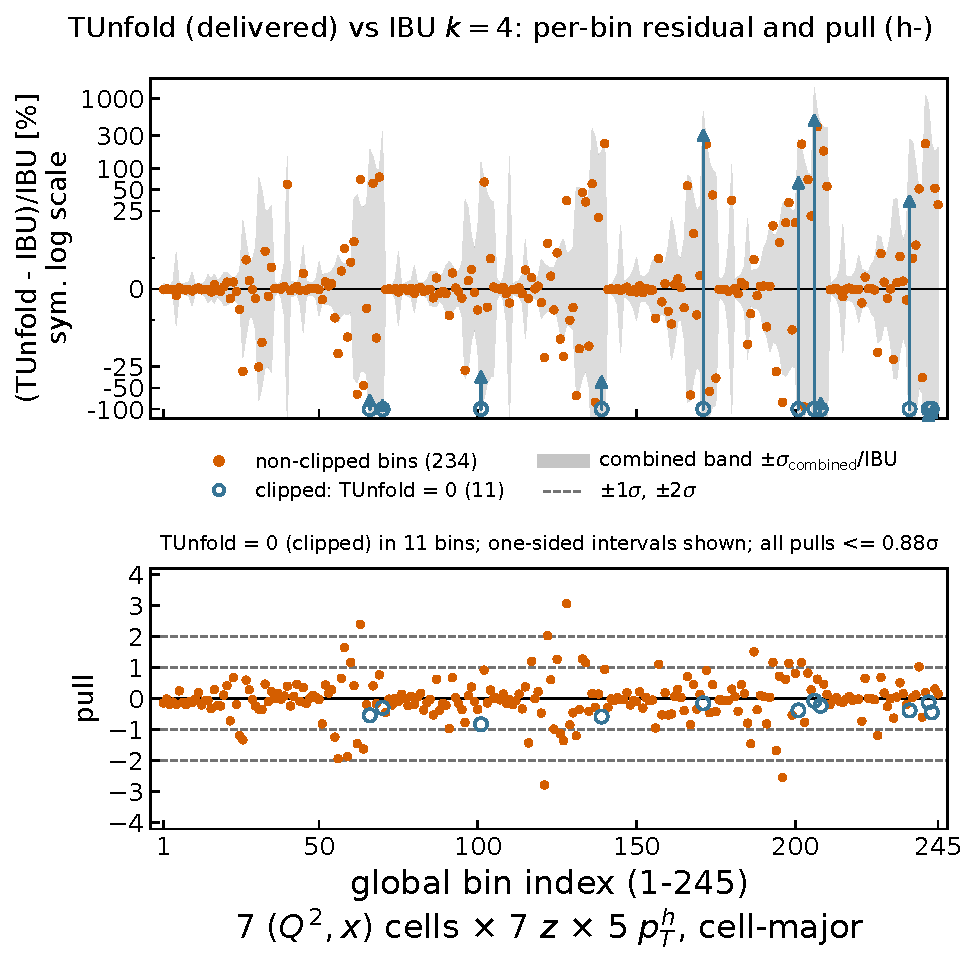
\includegraphics[width=\textwidth]{figures/fig_unfolding_tunfold_vs_ibu_residualpull_z005_hminus.pdf}
    \caption{$\hminus$.}
  \end{subfigure}
  \caption{Residuals and pulls by global bin index for the raw-level superseded-basis TUnfold diagnostic.  TUnfold uses $\tau=10^{-5}$ with delivered value $\max(x,0)$; clipped bins are open at $-100\%$ with one-sided interval bars.  Here $\mathrm{pull}=(x_{\mathrm{TU}}-x_{\mathrm{IBU}})/\sigma_{\mathrm{combined}}$.  The comparison is retained as a diagnostic cross-check with the iterative Bayesian unfolding as nominal; all 25 zero-delivered bins are statistically compatible with IBU, with maximum combined pulls of $1.21\sigma$ ($h^+$) and $0.88\sigma$ ($h^-$).}
  \label{fig:unfolding:tunfold-vs-ibu-residualpull}
\end{figure}

\begin{figure}[t]
  \centering
  \begin{subfigure}[t]{0.49\textwidth}
    \centering
    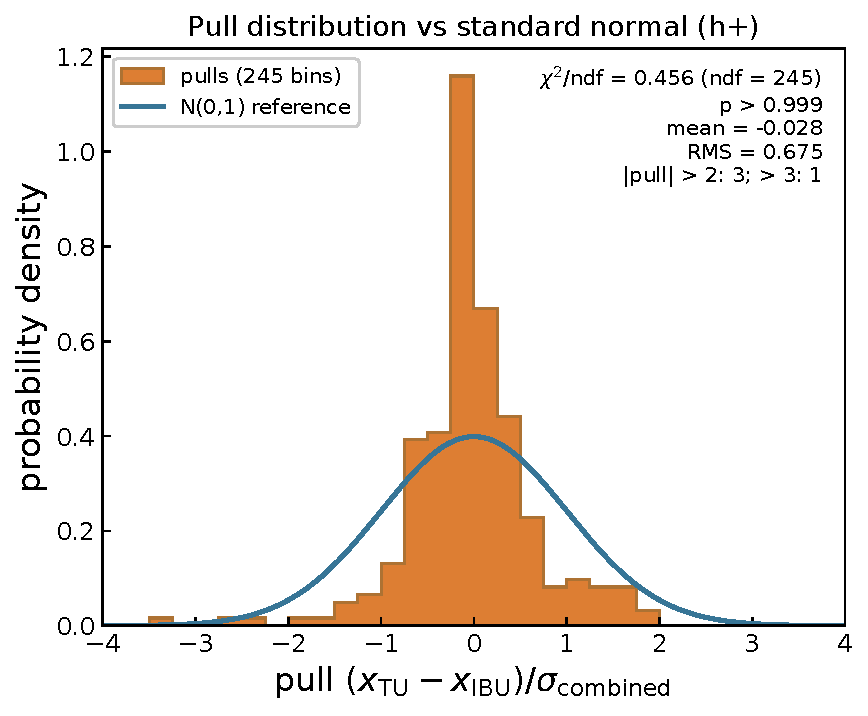
\includegraphics[width=\textwidth]{figures/fig_unfolding_tunfold_vs_ibu_pulls_z005_hplus.pdf}
    \caption{$\hplus$.}
  \end{subfigure}
  \hfill
  \begin{subfigure}[t]{0.49\textwidth}
    \centering
    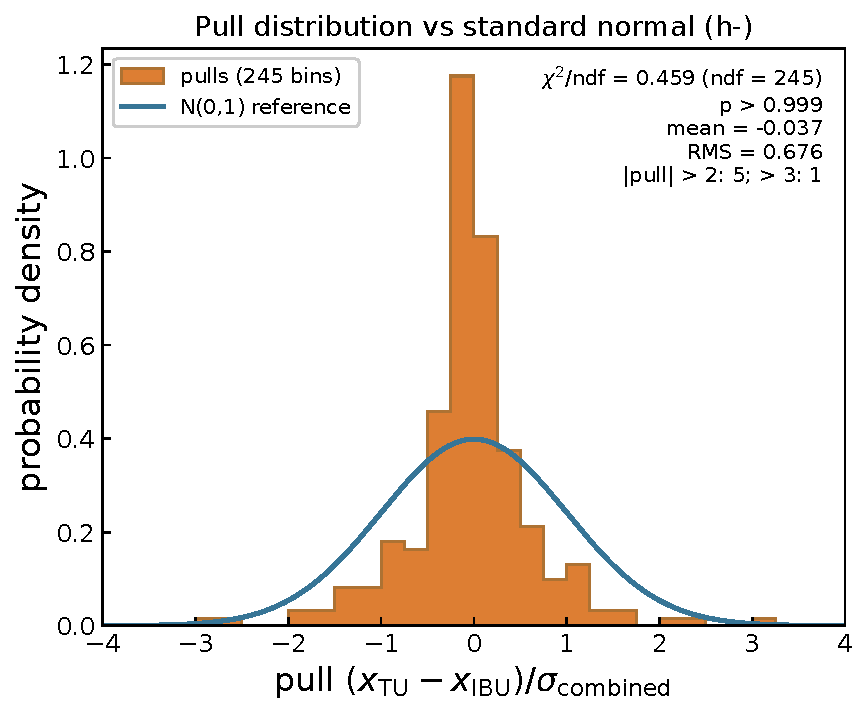
\includegraphics[width=\textwidth]{figures/fig_unfolding_tunfold_vs_ibu_pulls_z005_hminus.pdf}
    \caption{$\hminus$.}
  \end{subfigure}
  \caption{Distribution of $\mathrm{pull}=(x_{\mathrm{TU}}-x_{\mathrm{IBU}})/\sigma_{\mathrm{combined}}$ for the raw-level superseded-basis TUnfold diagnostic, compared with a standard-normal reference.  TUnfold uses $\tau=10^{-5}$ and the delivered prescription $\max(x,0)$; the comparison is retained as a diagnostic cross-check while the iterative Bayesian unfolding is nominal.  The diagonal-covariance consistency values are $\chi^2/\mathrm{ndf}=0.456$ and 0.459 for $h^+$ and $h^-$, with $p>0.999$.}
  \label{fig:unfolding:tunfold-vs-ibu-pulls}
\end{figure}


